\section{Narzędzie do porównywania wydajności i model bazy }

W rozdziale zostanie przedstawiona aplikacja umożliwiająca przeprowadzenie testów wybranych baz danych. Pokazana zostanie struktura testowej bazy danych oraz opisane zostaną przeprowadzane testy.

\subsection{Aplikacja}

W celu przeprowadzenia testów wybranych baz danych stworzona została aplikacja umożliwiająca przetestowanie szybkości baz danych w systemie iOS. Na rysunku 4.1 znajdującym się poniżej pokazany został pierwszy ekran aplikacji umożliwiający wybranie baz danych do testów. 

\begin{figure}[h]
\centering
	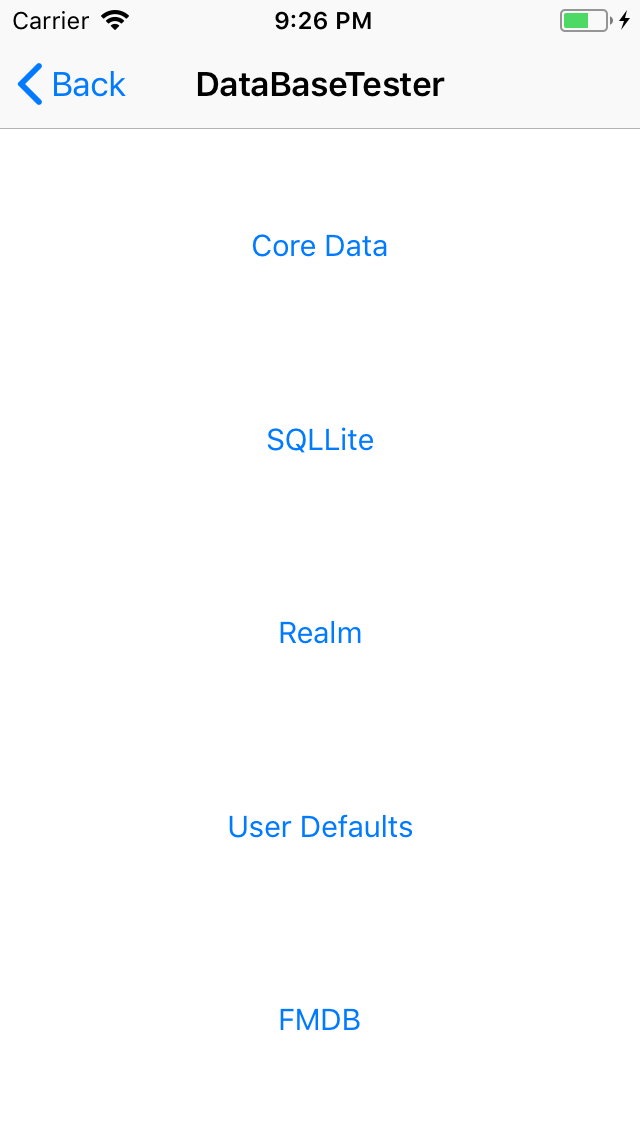
\includegraphics[width=6cm]{img/application/app-first-view.png}
	\caption{Ekran wyboru bazy danych do testów}
	\label{fig: first_app_view}
\end{figure}

Po wyborze bazy danych użytkownik zostaje przeniesiony do kolejnego ekranu aplikacji w którym należy wybrać jeden z dostępnych testów. Ekran widoczny jest na rysunku 4.2 znajdującym się poniżej.

\begin{figure}[h]
\centering
	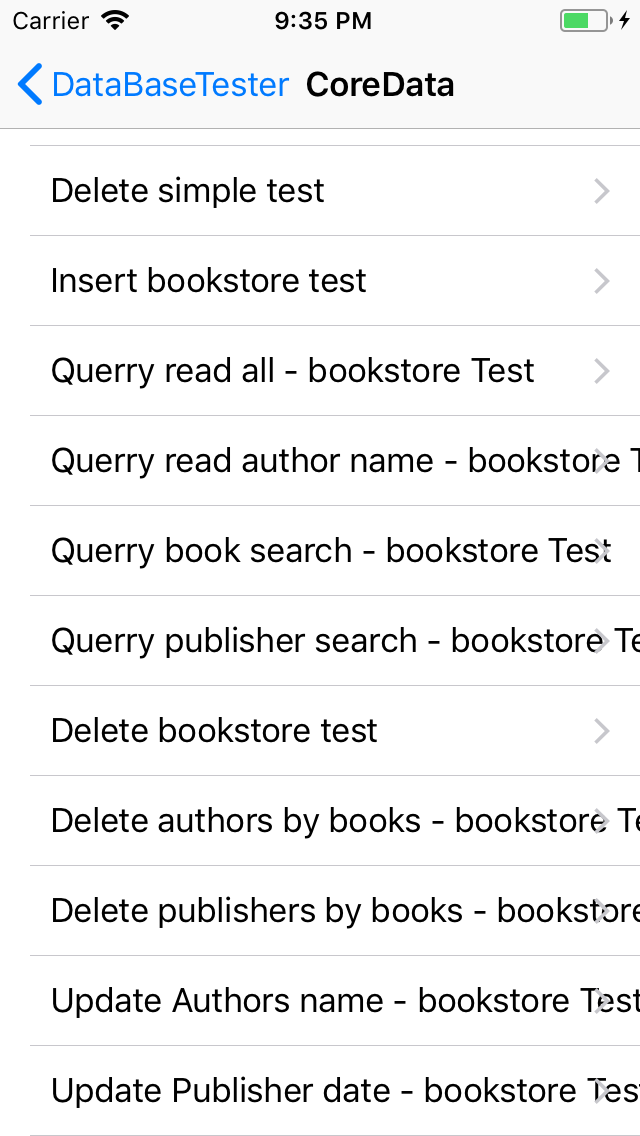
\includegraphics[width=6cm]{img/application/app-second-view.png}
	\caption{Ekran wyboru testu bazy danych}
	\label{fig: second_app_view}
\end{figure}

\newpage

Po wyborze jednego z testów następuje przejście do kolejnego ekranu widocznego na rysunku 4.3. Jest to ekran wyboru parametrów testu takich jak wielkość zestawu danych testowych i ilości powtórzeń testu. 

\begin{figure}[h]
\centering
	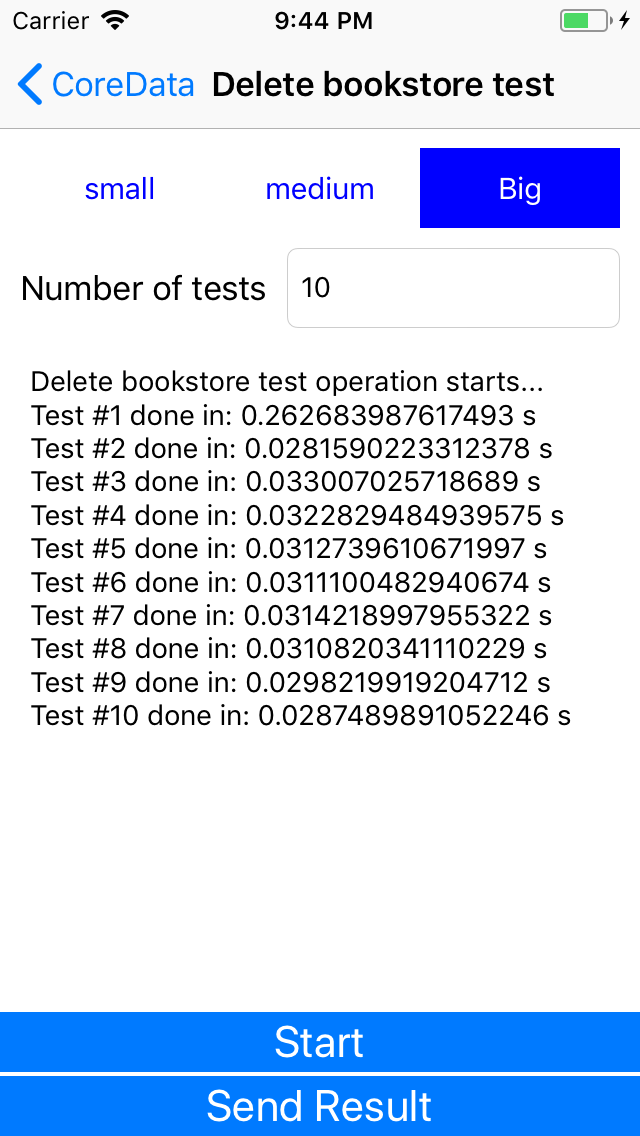
\includegraphics[width=6cm]{img/application/app_third-view.png}
	\caption{Ekran wykonywania testu}
	\label{fig: third_app_view}
\end{figure}

\newpage

Na ekranie znajduje się przycisk "Start" który uruchamia test. Podczas wykonywania testu na ekranie wypisywane są czasy w których zakończone zostają pojedyncze iteracje. Kiedy test dobiegnie końca za pomocą przycisku "Send Result" możliwa jest generacja pliku CSV zawierającego wszystkie uzyskane wyniki takie jak czasy pojedynczych operacji, użycie pamięci operacyjnej aplikacji podczas trwania testu czy też użycie procesora podczas każdej z przeprowadzanych operacji. 

\subsection{Schemat bazy danych}

Do przeprowadzenia testów zaprojektowany został prosty schemat bazy danych. Widoczny jest na rysunku 4.4. Zawiera on następujące tablice: Autor, Książka, Wydawnictwo. Autor może mieć wiele książek zaś książka wielu autorów - użyta została tu relacja wiele do wielu. Wydawnictwo może wiele książek ale jedna książka może mieć tylko jedno wydawnictwo - zastosowana została relacja jeden do wielu. 

\begin{figure}[h]
\centering
	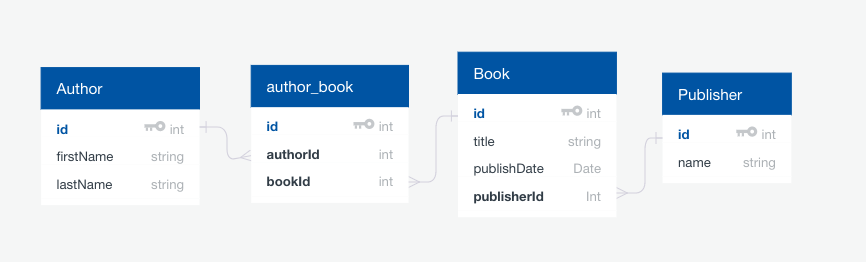
\includegraphics[width=\linewidth]{img/database/sql-scheme.png}
	\caption{Schemat basy danych SQL}
	\label{fig: sql_data_schame}
\end{figure}

Zaprojektowany schemat bazy umożliwia przetestowanie działania baz danych przy pracy na tabelach w których są różne typy relacji a także zapewnia możliwość testowania odczytu i zapisu daty. Data jest jednym z ważniejszych elementów w mobilnych bazach danych ponieważ niektóre rozwiązania bazodanowe nie zapewniają wsparcia dla tego formatu danych o czym była mowa podczas opisu wybranych baz danych. \par 

W pracy zostały użyte różne typy baz danych a mianowicie bazy NoSQL. Dla Realm i Core Data stworzony został schemat bazy widoczny na rysunku 4.5, nie posiadający tablicy pośredniej dla relacji wiele do wielu (Autor - Książka). Tablica ta jest zbędna dla tego typu baz danych ponieważ relacja wiele do wielu przechowywana jest za pomocą listy książek w tabeli autor i listy autorów w tablicy książka. 

\begin{figure}[h]
\centering
	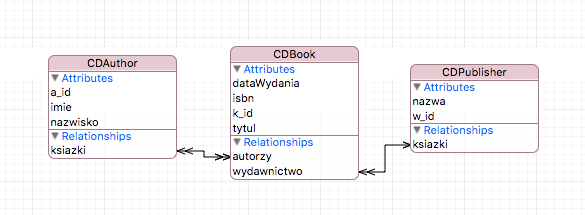
\includegraphics[width=\linewidth]{img/database/document-sheme.png}
	\caption{Schemat basy danych dla Realm i Core Data}
	\label{fig: nosql_data_scheme}
\end{figure}

Dla domyślnej bazy użytkownika - User Defaults struktura zapisywanych obiektów wygląda tak samo jak schemat dla baz NoSQL widoczny na rysunku 4.5. \par 

\section{Opis przeprowadzonych testów}

W rozdziale zostały opisane testy przeprowadzone w ramach pracy. Przedstawiono kroki potrzebne do otrzymania poprawnych wyników w zależności od typu testu oraz pokazano w jaki sposób został mierzony czas uzyskania rezultatu każdej operacji. 

\subsection{Testowane operacje}

W ramach analizy zostały przetestowane operacje CRUD - zapis, odczyt, uaktualnienie i usuwanie danych. W celu uzyskania jak najbardziej poprawnych wyników testy zostały przeprowadzone stukrotnie a wyniki przedstawiane w analizie są uśrednieniem wszystkich stu operacji dla danego testu. Przeprowadzenie operacji więcej niż jeden raz ma ogromne znaczenie ponieważ otrzymane czasy operacji zależne są od obciążenia urządzenia w danym czasie. Wszystkie testy zostały przeprowadzone na  urządzeniu iPhone 6s. \par

Testy były przeprowadzone dla następujących operacji: 
\begin{itemize}
	 \item Zapis
  
  	\begin{itemize}
    		\item Zapisz wszystkich danych do bazy
	 \end{itemize}

	  \item Odczyt
	  
   	  \begin{itemize}
   		 \item Odczyt wszystkich danych z tabel
	     \item Wyszukanie wszystkich autorów o imieniu "Diena"
   		 \item Wyszukanie 2 książek z największa liczbą autorów
     	\item Odczyt maksymalnie 20 wydawnictw z największą liczba wydanych książek i posortowanie wyniku rosnąco   
  		\end{itemize}
  		
 	  \item Edycja

 	  	\begin{itemize}
	    		\item Edycja imienia autora "Diena" na "Alona"
	    		\item Edycja daty wydania książek na obecna datę
		 \end{itemize}

	   \item Usuwanie
	   
	    	\begin{itemize}
	    		\item Usunięcie wszystkich danych
	    		\item Usunięcie wszystkich autorów którzy wydali 3 książki
	    		\item Usunięcie wydawnictw które wydały książki o tytułach "Annie Oakley" lub "Tokyo Zombie (Tky zonbi)"
		 \end{itemize}	 
\end{itemize}

W celu otrzymania dokładnych wyników świadczących o wydajności bazy danych testy były projektowane tak aby operowały one na wszystkich danych zawartych w tabelach a także na niektórych z wybranych podczas zapytania. Zapewnia to lepszy obraz wydajności bazy danych kiedy istnieje potrzeba przetworzenia wszystkich danych w danej tabeli lub kiedy należy przeprowadzić operacje na kilku rekordach. 

\subsection{Dane testowe}

Jak wspomniano w rozdziale  4 podczas opisu aplikacji, przed wykonaniem testu możliwy jest wybór zestawu danych testowych. Zestaw duży to tysiąc danych, zestaw średni to sto danych testowych a zestaw mały to 10 danych. Liczba danych dla każdej z tabel (Autor, Książka, Wydawnictwo) w zależności od wielkości zestawu danych przedstawiony został w tabeli \ref{tab: zestaw_danych}.

\begin{table}[h]
\centering
\caption {Liczba rekordów w zestawach danych testowych}
\label{tab: zestaw_danych}
\begin{tabular}{|c|c|c|c|}
\hline
\multicolumn{1}{|l|}{} & Mały & Średni & Duży \\ \hline
Wydawnictwo            & 1    & 10     & 100  \\ \hline
Książka                & 6    & 60     & 600  \\ \hline
Autor                  & 3    & 30     & 300  \\ \hline
\end{tabular}
\end{table}

Różna ilości danych ma na celu pokazanie podczas testów zmian wydajności każdej z baz. Każda z baz inaczej będzie sobie radzić z różną ilością danych. Dane testowe zostały wygenerowane za pomocą serwisu internetowego MOCKAROO. 

\subsection{Przebieg testów}

W pracy skupiono się na wydajności baz danych, ale z powodu testowania różnego typu baz należało przyjąć odpowiednie zasady testów.\par 
Bazy Core Data czy Realm w wyniku zapytania zwracają obiekty, różniące się od siebie pod względem implementacji ale zawierające te same pola zawarte w modelu bazy. Różnice te wynikają z różnego sposobu działania baz danych, przedstawione one zostały w kolejnych rozdziałach pracy. Bazy SQLite i FMBD w rezultacie zapytania zwracają surowe dane a nie obiekty. Jasne staje się że czasy otrzymania obiektu względem otrzymania surowego rezultatu będą różne. Aby otrzymać miarodajne rezultaty testów założono więc, że wynikiem końcowym każdego z testów odczytu będzie otrzymanie listy obiektów programu a nie samych surowych danych. 

\begin{figure}[h]
\centering
	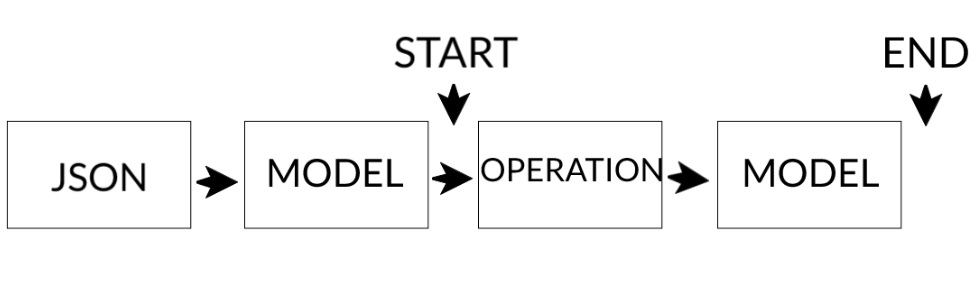
\includegraphics[width=\linewidth]{img/database/operation-scheme.png}
	\caption{Przebieg testów}
	\label{fig: operation_scheme}
\end{figure}

Cały proces testów przedstawia rysunek 5.1.  Pierwszym etapem jest przekształcenie plików w formacie JSON na obiekty programu, których typ jest zależny od wybranej bazy danych. Kolejny z etapów to przekazanie obiektów do odpowiedniej bazy danych i zaczęcie wykonywania operacji, od tego momentu mierzony jest czas operacji. Po wykonaniu operacji otrzymany rezultat operacji przekształcany jest ponownie na obiekty programu i po zakończeniu tej operacji następuje koniec pomiaru czasu operacji. 

W zależności od typu badanej operacji zastosowane zostały różne scenariusze testów. Zależnie od operacji można rozróżnić trzy typy scenariuszy: 

\begin{itemize}
	 \item Zapis danych - w pętli wykonywane są następujące operacje:
	 
	 \begin{enumerate}
	 \item Wygenerowanie danych
	 \item Wyczyszczenie bazy danych
	 \item Wykonanie zapisu danych do bazy
	 \end{enumerate}
	 
	 \item Odczyt danych:
	 
	  \begin{enumerate}
	 \item Wygenerowanie danych
	 \item Wyczyszczenie bazy danych
	 \item Wykonanie zapisu danych do bazy
	 \item W pętli wykonywana zostaje operacja odczytania danych i pomiar czasów
	 \end{enumerate}
	 
	 \item Usuwanie i edycja danych - w pętli wykonywane są następujące operacje:
	 
	 \begin{enumerate}
	 \item Wygenerowanie danych
	 \item Wyczyszczenie bazy danych
	 \item Wykonanie zapisu danych do bazy
	 \item Wykonanie operacji usuwania lub edycji danych i pomiar czasów
	 \end{enumerate}
	 
\end{itemize}

Ilość wykonywania powtórzeń operacji poprzez pętle zostaje zdefiniowana przez użytkownika w ekranie aplikacji widocznym na rysunku \ref{fig: third_app_view}, poprzez wprowadzenie liczby testów w polu tekstowym. Jak można zauważyć najbardziej czasochłonnymi testami jest pomiar czasu edycji i usuwania danych. Podczas tego testu wielokrotnie jest powtarzana operacja zapisu do danych.  